\section{Phân tích độ phức tạp}\label{Appendix:Complexity}
Chi phí tính toán của khung QCAD của chúng tôi chủ yếu đến từ hai phần: tính toán ma trận Khoảng cách của Gower bằng cách sử dụng các đặc trưng ngữ cảnh và tính toán điểm bất thường bằng cách sử dụng tất cả các tính năng dựa trên Rừng hồi quy phân vị.

Độ phức tạp về thời gian của việc tính toán ma trận Khoảng cách của Gower là $O(N^{2}D_{cnt})$, trong đó $N$ biểu thị kích thước mẫu và $D_{cnt}$ biểu thị số lượng đặc trưng ngữ cảnh. Ngoài ra, độ phức tạp về thời gian của việc xây dựng một khu rừng ngẫu nhiên là $O( n_{tree}\cdot n_{feature} \cdot k log(k))$ và sử dụng nó để dự đoán là $O( n_{tree}\cdot n_{feature})$ \citep{buczak2015survey}, trong đó $n_{tree}$ là số cây được sử dụng để tạo thành một khu rừng ngẫu nhiên, $n_{feature}$ biểu thị số thứ nguyên (tức là nhiều nhất là $D_{cnt}$) và $k$ cho biết số lượng mẫu được sử dụng để xây dựng khu rừng (tức là số lượng hàng xóm gần nhất trong trường hợp của chúng tôi). Do đó, độ phức tạp về thời gian của việc xây dựng các khu rừng hồi quy phân vị $N$ trong các đặc trưng hành vi của $D_{bhv}$ là $O( n_{tree}\cdot D_{cnt} \cdot k log(k) \cdot N \cdot D_{bhv} )$.
Hơn nữa, chúng tôi phải ước tính $100$ các lượng tử khác nhau bằng cách sử dụng từng rừng hồi quy phân vị, dẫn đến $O( (n_{tree} \cdot D_{cnt} \cdot k log(k)+ n_{tree} \cdot D_{cnt} \cdot 100) \cdot N \cdot D_{bhv} )$. Do đó, việc sử dụng cài đặt mặc định của chúng tôi sẽ dẫn đến $O( ( 100 \cdot D_{cnt} \cdot \mathrm{min}(500,\frac{N}{2})\cdot \mathrm{log}(\mathrm{min}(500,\frac{N}{2})) + 100 \cdot D_{cnt} \cdot 100) \cdot N \cdot D_{bhv})$. Trường hợp xấu nhất là $O(10^{5}N D_{cnt}D_{bhv}).$

Nhìn chung, độ phức tạp về thời gian của phương pháp của chúng tôi là $O(10^{5}N D_{cnt}D_{bhv}+N^{2}D_{cnt})$ trong trường hợp xấu nhất. Đặc biệt, độ phức tạp về thời gian trở thành $O(10^{5}N D_{cnt}D_{bhv})$ khi $N<10^{5}$ (tức là đối với các tập dữ liệu vừa và nhỏ). Ngoài ra, việc xây dựng các khu rừng hồi quy phân vị cho từng đối tượng trong từng đặc trưng hành vi có thể dễ dàng được thực hiện theo cách song song, do đó giảm độ phức tạp về thời gian xuống $O(10^{5}N D_{cnt}+N^{2}D_{cnt})$ trong trường hợp xấu nhất.

\section{Mô tả tập dữ liệu}\label{Appendix:Data}

\paragraph{Bào ngư} Tập dữ liệu chứa các bản ghi đo vật lý bào ngư 4177. Cụ thể, chúng tôi sử dụng các đặc điểm Giới tính, Chiều dài, Đường kính và Chiều cao làm đặc trưng ngữ cảnh. Theo đó, chúng tôi sử dụng các đặc điểm Trọng lượng Toàn bộ, Trọng lượng Shucked, Trọng lượng Nội tạng, Trọng lượng Vỏ và Vòng làm các đặc trưng hành vi. Tập dữ liệu này được tải xuống từ UCI, \footnote{https://archive.ics.uci.edu/ml/datasets/abalone} không chứa giá trị nào bị thiếu.


\paragraph{Độ ồn của cánh máy bay} Tập dữ liệu này chứa các bản ghi 1503 từ một loạt các thử nghiệm khí động học và âm thanh của các phần cánh cánh máy bay. Cụ thể, chúng tôi sử dụng các tính năng mô tả tần số, góc tấn công, độ dài hợp âm, vận tốc dòng tự do và độ dày dịch chuyển phía hút (ví dụ: f, alpha, c, U\_infinity và delta) làm các đặc trưng ngữ cảnh. Trong khi đó, tính năng mô tả mức áp suất âm thanh được chia tỷ lệ (ví dụ: SSPL) là đặc trưng hành vi. Tập dữ liệu này được tải xuống từ UCI, \footnote{https://archive.ics.uci.edu/ml/datasets/Airfoil+Self-Noise} không chứa giá trị nào bị thiếu.\paragraph{Bodyfat} Tập dữ liệu này chứa các ước tính về mật độ cơ thể và
tỷ lệ phần trăm mỡ cơ thể (được sử dụng làm đặc trưng hành vi), được xác định bằng nhiều phép đo chu vi cơ thể khác nhau, chẳng hạn như Tuổi, Cân nặng, Chiều cao, Chu vi cổ, Chu vi ngực, Chu vi bụng 2, Chu vi hông, Chu vi đùi, Chu vi đầu gối, Chu vi mắt cá chân, Chu vi bắp tay (mở rộng), Chu vi cẳng tay và Chu vi cổ tay (được sử dụng làm đặc trưng ngữ cảnh) cho nam giới 252. Tập dữ liệu thô không bao gồm các tính năng phân loại và các giá trị bị thiếu 0, được tải xuống từ statlib CMU. \footnote{http://lib.stat.cmu.edu/datasets/bodyfat}


\paragraph{Giá nhà ở Boston} Tập dữ liệu này chứa các bản ghi 583 về giá nhà ở Boston. Chúng tôi sử dụng các đặc điểm mô tả các thuộc tính của ngôi nhà và môi trường xung quanh nó, ví dụ: CRIM, ZN, INDUS, CHAS, NOX, RM, AGE, DIS, RAD, TAX, PTRATIO, B, LSTAT làm đặc điểm ngữ cảnh và giá trị trung bình của các ngôi nhà do chủ sở hữu sử dụng, tức là MED, làm đặc trưng hành vi. Tập dữ liệu này được phát hành bởi \cite{harrison1978hedonic} và được tải xuống từ CMU statlib \footnote{http://lib.stat.cmu.edu/datasets}. Nó vẫn giữ lại các bản ghi 506 sau khi loại bỏ các hàng chứa giá trị bị thiếu.

\paragraph{Cường độ nén bê tông } Tập dữ liệu này chứa các bản ghi 1030 về cường độ nén của bê tông. Chúng tôi sử dụng các đặc điểm mô tả độ tuổi và các thành phần khác nhau làm đặc trưng ngữ cảnh, bao gồm C1, C2, C3, C4, C5, C6, C7 và Tuổi. Ngoài ra, chúng tôi sử dụng tính năng Strength làm đặc trưng hành vi. Tập dữ liệu này được tải xuống từ UCI, \footnote{https://archive.ics.uci.edu/ml/datasets/Concrete+Compressive+Strength} không chứa giá trị bị thiếu.

\paragraph{El Nino } Tập dữ liệu này chứa các bản ghi 178080 về các chỉ số khí tượng bề mặt và hải dương học, đó là
lấy từ các phao nằm khắp vùng xích đạo Thái Bình Dương. Chúng tôi sử dụng các tính năng không gian và thời gian, ví dụ: Năm, Tháng, Ngày, Ngày, Vĩ độ, Kinh độ làm các đặc trưng ngữ cảnh và các tính năng khác, ví dụ: Zonal\_Winds, Meridional\_Winds, Độ ẩm, Air\_Temp, Sea\_Surface\_Temp là các đặc trưng hành vi. Tập dữ liệu này được tải xuống từ kho lưu trữ máy học UCI.\footnote{archive.ics.uci.edu/ml/datasets/El+Nino}. Tập dữ liệu này vẫn giữ lại các bản ghi 93935 sau khi loại bỏ các hàng chứa các giá trị bị thiếu. Tuy nhiên, để tất cả các thuật toán hoàn thành thử nghiệm trên tập dữ liệu này trong vòng vài giờ 12, chúng tôi lấy mẫu ngẫu nhiên tập dữ liệu gốc xuống bản ghi 20,000.

\paragraph{Energy Efficiency} Tập dữ liệu này chứa các bản ghi 768 về một nghiên cứu đánh giá hiệu quả năng lượng như một hàm của các thông số tòa nhà. Theo đó, các tham số của tòa nhà như X1, X2, X3, X4, X5, X6, X7 và X8 được coi là các đặc trưng ngữ cảnh, còn tải sưởi ấm và tải làm mát (cụ thể là Y1 và Y2) được coi là các đặc trưng hành vi. Tập dữ liệu này được tải xuống từ UCI, \footnote{https://archive.ics.uci.edu/ml/datasets/Energy+efficiency} không chứa giá trị nào bị thiếu.\paragraph{Trọng lượng cá } Tập dữ liệu này chứa các bản ghi 157 về đặc điểm của các loài cá phổ biến trên thị trường. Theo đó, chúng tôi sử dụng các đặc điểm bao gồm Loài, Chiều dài1, Chiều dài2, Chiều dài3, Chiều cao, Chiều rộng làm đặc trưng ngữ cảnh và Trọng lượng làm đặc trưng hành vi. Tập dữ liệu này được tải xuống từ Kaggle, \footnote{https://www.kaggle.com/aungpyaeap/fish-market} không chứa giá trị nào bị thiếu.

\paragraph{Cháy rừng} Tập dữ liệu này chứa các bản ghi 517 liên quan đến thông tin khí tượng và không gian thời gian về cháy rừng ở khu vực đông bắc Bồ Đào Nha. Chúng tôi sử dụng các đặc điểm không gian theo thời gian như X, Y, tháng, ngày làm các đặc trưng ngữ cảnh và các đặc điểm còn lại, tức là FFMC, DMC, DC, ISI, nhiệt độ, RH, gió, mưa, khu vực làm các đặc trưng hành vi. Nó được tải xuống từ kho lưu trữ máy học UCI,\footnote{https://archive.ics.uci.edu/ml/datasets/forest+fires} không chứa giá trị nào bị thiếu.

\paragraph{Phát thải CO và NOx của tuabin khí } Tập dữ liệu ban đầu bao gồm các bản ghi 36733 về dữ liệu đo cảm biến, được thu thập từ một tuabin khí ở Thổ Nhĩ Kỳ từ 2011 đến 2015. Bộ dữ liệu được thu thập từ cùng một nhà máy điện để nghiên cứu lượng khí thải và dự đoán sản lượng năng lượng ròng hàng giờ. Do đó, chúng tôi sử dụng các tính năng mô tả các tham số tuabin (ví dụ: AT, AP, AH, AFDP, GTEP, TIT, TAT và CDP) làm các đặc trưng ngữ cảnh.
Các biến đặc trưng cho hiệu suất năng lượng của tuabin và lượng phát thải khí (ví dụ: TEY, CO và NOX) được sử dụng làm đặc trưng hành vi. Tuy nhiên, để tất cả các thuật toán hoàn thành thử nghiệm trong vòng 12 giờ, chúng tôi chỉ sử dụng các bản ghi 7383 trong 2015. Tập dữ liệu này được tải xuống từ UCI, \footnote{https://archive.ics.uci.edu/ml/datasets/Gas+Turbine+CO+and+NOx+Emission+Data+Set} không chứa giá trị bị thiếu.


\paragraph{Suy tim}
Tập dữ liệu này chứa hồ sơ lâm sàng về bệnh suy tim của bệnh nhân 299 bị suy tim. Nó chứa các đặc điểm lâm sàng 13, trong đó chúng tôi sử dụng tuổi tác, giới tính, hút thuốc, bệnh tiểu đường, \_blood\_áp lực và thiếu máu làm đặc trưng ngữ cảnh và creatinine\_phosphokinase, ejection\_phân đoạn, tiểu cầu, huyết thanh\_creatinine, huyết thanh\_sodium, thời gian là đặc trưng hành vi. Ngoài ra, tính năng death\_event đã bị xóa và không có giá trị nào bị thiếu trong tập dữ liệu này. Tập dữ liệu gốc được phát hành bởi \cite{ahmad2017survival} và chúng tôi tải xuống từ kho lưu trữ máy học UCI. \footnote{archive.ics.uci.edu/ml/datasets/Heart+failure+clinical+records}

\paragraph{Viêm gan}
Tập dữ liệu này chứa các bản ghi 615 liên quan đến giá trị xét nghiệm của người hiến máu và bệnh nhân Viêm gan C. Chúng tôi sử dụng các đặc điểm nhân khẩu học như giới tính và độ tuổi cũng như Danh mục nhà tài trợ làm đặc điểm ngữ cảnh và các đặc điểm còn lại, tức là ALB, ALP, ALT, AST, BIL, CHE, CHOL, CREA, GGT và PROT làm đặc trưng hành vi. Tập dữ liệu gốc được tải xuống từ Kho lưu trữ máy học UCI. \footnote{ https://archive.ics.uci.edu/ml/datasets/HCV+data} Bản ghi 26 chứa các giá trị bị thiếu và do đó bị xóa.\paragraph{Bệnh nhân gan Ấn Độ}
Tập dữ liệu này chứa hồ sơ y tế của bệnh nhân gan Ấn Độ 583, 4 chứa các giá trị bị thiếu và do đó bị xóa khỏi phân tích sâu hơn. Chúng tôi coi Độ tuổi, Giới tính và Bộ chọn là các đặc trưng ngữ cảnh và Total\_Bilirubin, Direct\_Bilirubin, Alkaline\_Phosphotase, Alamine\_Aminotransferase, Aspartate\_Aminotransferase, Total\_Protiens, Albumin, Albumin\_and\_Globulin\_Ratio là các đặc trưng hành vi. Tập dữ liệu này được tải xuống từ kho lưu trữ máy học của UCI. \footnote{https://archive.ics.uci.edu/ml/datasets/ILPD+(Indian+Liver+Patient+Dataset)}

\paragraph{Bảo trì các nhà máy động cơ đẩy hải quân } Bộ dữ liệu chứa các bản ghi thử nghiệm 11934, được thực hiện bằng mô phỏng số của một tàu hải quân có nhà máy động cơ đẩy tua-bin khí. Chúng tôi sử dụng các tính năng mô tả các biện pháp tuabin khí của tài sản vật chất làm các đặc trưng ngữ cảnh, bao gồm LeverPosition, GTT, GTn, GGn, Ts, Tp, T48, T1, T2, P48, P1, P2, Pexh, TIC, mf. Trong khi đó, chúng tôi sử dụng các đặc điểm chứa tốc độ tàu và sự suy giảm hiệu suất theo thời gian của các bộ phận tuabin khí, ví dụ: ShipSpeed, CompressorDecay và TurbineDecay, làm các đặc trưng hành vi. Tập dữ liệu này được tải xuống từ UCI, \footnote{https://archive.ics.uci.edu/ml/datasets/Condition+Based+Maintenance+of+Naval+Propulsion+Plants} không chứa giá trị bị thiếu.

\paragraph{Parkinsons Telemonitoring} Bộ dữ liệu chứa các bản ghi 5875 của một loạt phép đo giọng nói y sinh từ các bệnh nhân mắc bệnh Parkinson giai đoạn đầu 42. Ở đó, mọi người được tuyển vào cuộc thử nghiệm kéo dài sáu tháng về thiết bị giám sát từ xa để theo dõi tiến triển triệu chứng từ xa. Các tính năng như chủ đề, độ tuổi, giới tính, test\_time, Jitter, Jitter\_Abs, Jitter\_RAP, Jitter\_PPQ5, Jitter\_DDP, Shimmer, Shimmer\_dB, Shimmer\_APQ3, Shimmer\_APQ5, Shimmer\_APQ11, Shimmer\_DDA, NHR, HNR, RPDE, DFA, PPE mô tả thông tin cơ bản và do đó được sử dụng làm đặc trưng ngữ cảnh. Trong khi đó, điểm số tương ứng motor\_UPDRS và Total\_UPDRS được sử dụng làm đặc trưng hành vi. Tập dữ liệu này được tải xuống từ UCI, \footnote{https://archive.ics.uci.edu/ml/datasets/Parkinsons+Telemonitoring} không chứa giá trị nào bị thiếu.

\paragraph{Nhà máy điện} Tập dữ liệu này chứa các bản ghi 9568 từ một nhà máy điện chu trình hỗn hợp hoạt động ở mức đầy tải từ 2006 đến 2011. Các tính năng như nhiệt độ môi trường thay đổi trung bình hàng giờ, áp suất xung quanh, độ ẩm tương đối và chân không khí thải (ví dụ: T, AP, RH và EP) được coi là các đặc trưng ngữ cảnh, trong khi sản lượng điện thực hàng giờ (EP) được coi là đặc trưng hành vi. Tập dữ liệu này được tải xuống từ UCI, \footnote{https://archive.ics.uci.edu/ml/datasets/Combined+Cycle+Power+Plant} không chứa giá trị nào bị thiếu.\paragraph{Xếp hạng Đại học QS} Tập dữ liệu này chứa bảng xếp hạng QS của các trường đại học trên thế giới từ 2018 đến 2020. Chúng tôi xem xét thứ hạng thế giới, thứ hạng quốc gia và vị trí của từng trường đại học từ 2018 đến 2020, tức là World2018, National2018, World2019, National2019, World2020, National2020, Quốc gia là các đặc trưng ngữ cảnh. Chúng tôi sử dụng sáu đặc điểm được xem xét để xếp hạng (tức là Danh tiếng học thuật, Danh tiếng của nhà tuyển dụng, Tỷ lệ giảng viên trên sinh viên, Số lượng trích dẫn trên mỗi giảng viên, Khoa quốc tế, Sinh viên quốc tế) làm đặc trưng hành vi. Dữ liệu gốc được thu thập từ trang web QS, \footnote{https://www.topuniversities.com/qs-world-university-rankings} chứa các bản ghi 475 sau khi loại bỏ các giá trị bị thiếu.

\paragraph{QSAR Độc tính của cá} Tập dữ liệu này chứa các bản ghi 908 về cá Pimephales promelas. Cụ thể, sáu đặc điểm mô tả phân tử của hóa chất 908 sẽ được sử dụng làm đặc trưng ngữ cảnh và thước đo độc tính cấp tính đối với môi trường thủy sinh tương ứng sẽ được sử dụng làm đặc trưng hành vi. Tập dữ liệu này được tải xuống từ UCI, \footnote{https://archive.ics.uci.edu/ml/datasets/QSAR+fish+toxity} không chứa giá trị nào bị thiếu.

\paragraph{Máy đồng bộ } Tập dữ liệu này chứa các bản ghi 557 từ một bộ thử nghiệm thực. Thí nghiệm này nhằm mục đích xây dựng mô hình ước tính dòng điện kích thích của động cơ đồng bộ. Cụ thể, chúng tôi sử dụng các tính năng mô tả dòng điện tải, hệ số công suất, lỗi hệ số công suất và sự thay đổi của dòng điện kích thích (ví dụ: Iy, PF, e và dIf) làm các đặc trưng ngữ cảnh. Theo đó, đặc điểm mô tả
dòng kích thích của máy đồng bộ (cụ thể là If ) được sử dụng làm đặc tính hành vi. Tập dữ liệu này được tải xuống từ UCI, \footnote{https://archive.ics.uci.edu/ml/datasets/Synchronous+Machine+Data+Set} không chứa giá trị nào bị thiếu.


\paragraph{Du thuyền thủy động lực học } Tập dữ liệu này chứa các bản ghi 308 về các tính năng của du thuyền buồm. Chúng tôi sử dụng các tính năng mô tả kích thước, vận tốc và hiệu suất thủy động lực của du thuyền, cụ thể là Longitudinal\_position, Prismatic\_cofactor, length\_displacement\_ratio, Beam\_draught\_ratio, Số chiều dài\_beam\_ratio, Froude\_ là các đặc trưng ngữ cảnh và đặc điểm liên quan đến lực cản dư trên một đơn vị trọng lượng dịch chuyển, cụ thể là lực cản, là đặc trưng hành vi. Tập dữ liệu này được tải xuống từ kho lưu trữ máy học UCI, \footnote{archive.ics.uci.edu/ml/datasets/Yacht+Hydrodynamics} không chứa giá trị nào bị thiếu.

\section{Phân tích độ nhạy tham số}
\label{Appendix:Sensitivity}Thông số $k$ ảnh hưởng trực tiếp đến hiệu lực và hiệu quả của máy dò dị thường trong giai đoạn phát hiện bất thường. Nếu tập dữ liệu của chúng tôi được gắn nhãn, chúng tôi có thể sử dụng các kỹ thuật như tìm kiếm lưới và xác thực chéo để đặt $k$ tối ưu cho một tập dữ liệu cụ thể. Tuy nhiên, phát hiện bất thường thường là một vấn đề học tập không giám sát, khiến cho việc đặt $k$ tối ưu là không thể. Do đó, về mặt thực nghiệm, chúng tôi chỉ có thể đưa ra một số quy tắc kinh nghiệm để đặt $k$ theo các thuộc tính của tập dữ liệu cụ thể (ví dụ: cỡ mẫu, số chiều và tỷ lệ bất thường ước tính). Do đó, chúng tôi thực hiện các thử nghiệm chuyên sâu trên các bộ dữ liệu tổng hợp và trong thế giới thực với nhiều kích thước mẫu, số chiều và tỷ lệ dị thường được đưa vào để nghiên cứu độ nhạy của thuật toán của chúng tôi đối với tham số này.

Như được hiển thị trong Hình \ref{fig:sensitivity1}, việc tăng
số lượng hàng xóm, tức là $k$, sẽ dẫn đến hiệu suất tốt hơn về PRC AUC, ROC AUC và Precision@n khi $k$ nhỏ (khoảng $N/10$ cho hầu hết các tập dữ liệu). Tuy nhiên, mức tăng hiệu suất dần dần chậm lại khi $k$ tăng lên và hiệu suất cuối cùng đạt đến mức ổn định với mức tăng $k$. Sau đó, việc tăng thêm $k$ chỉ mang lại hiệu suất tăng không đáng kể và phải trả giá bằng thời gian chạy. Do đó, chúng tôi đặt $k$ thành $N/2$ cho tập dữ liệu nhỏ và $500$ cho tập dữ liệu trung bình sau khi cân nhắc giữa độ chính xác và chi phí thời gian chạy. Nhìn chung, khác với các máy dò dị thường dựa trên $k$-NN khác vốn nhạy cảm với tham số này, phương pháp QCAD của chúng tôi ổn định trên tham số $k$ miễn là giá trị của nó không quá nhỏ.

\begin{figure}[!htbp]
\centering
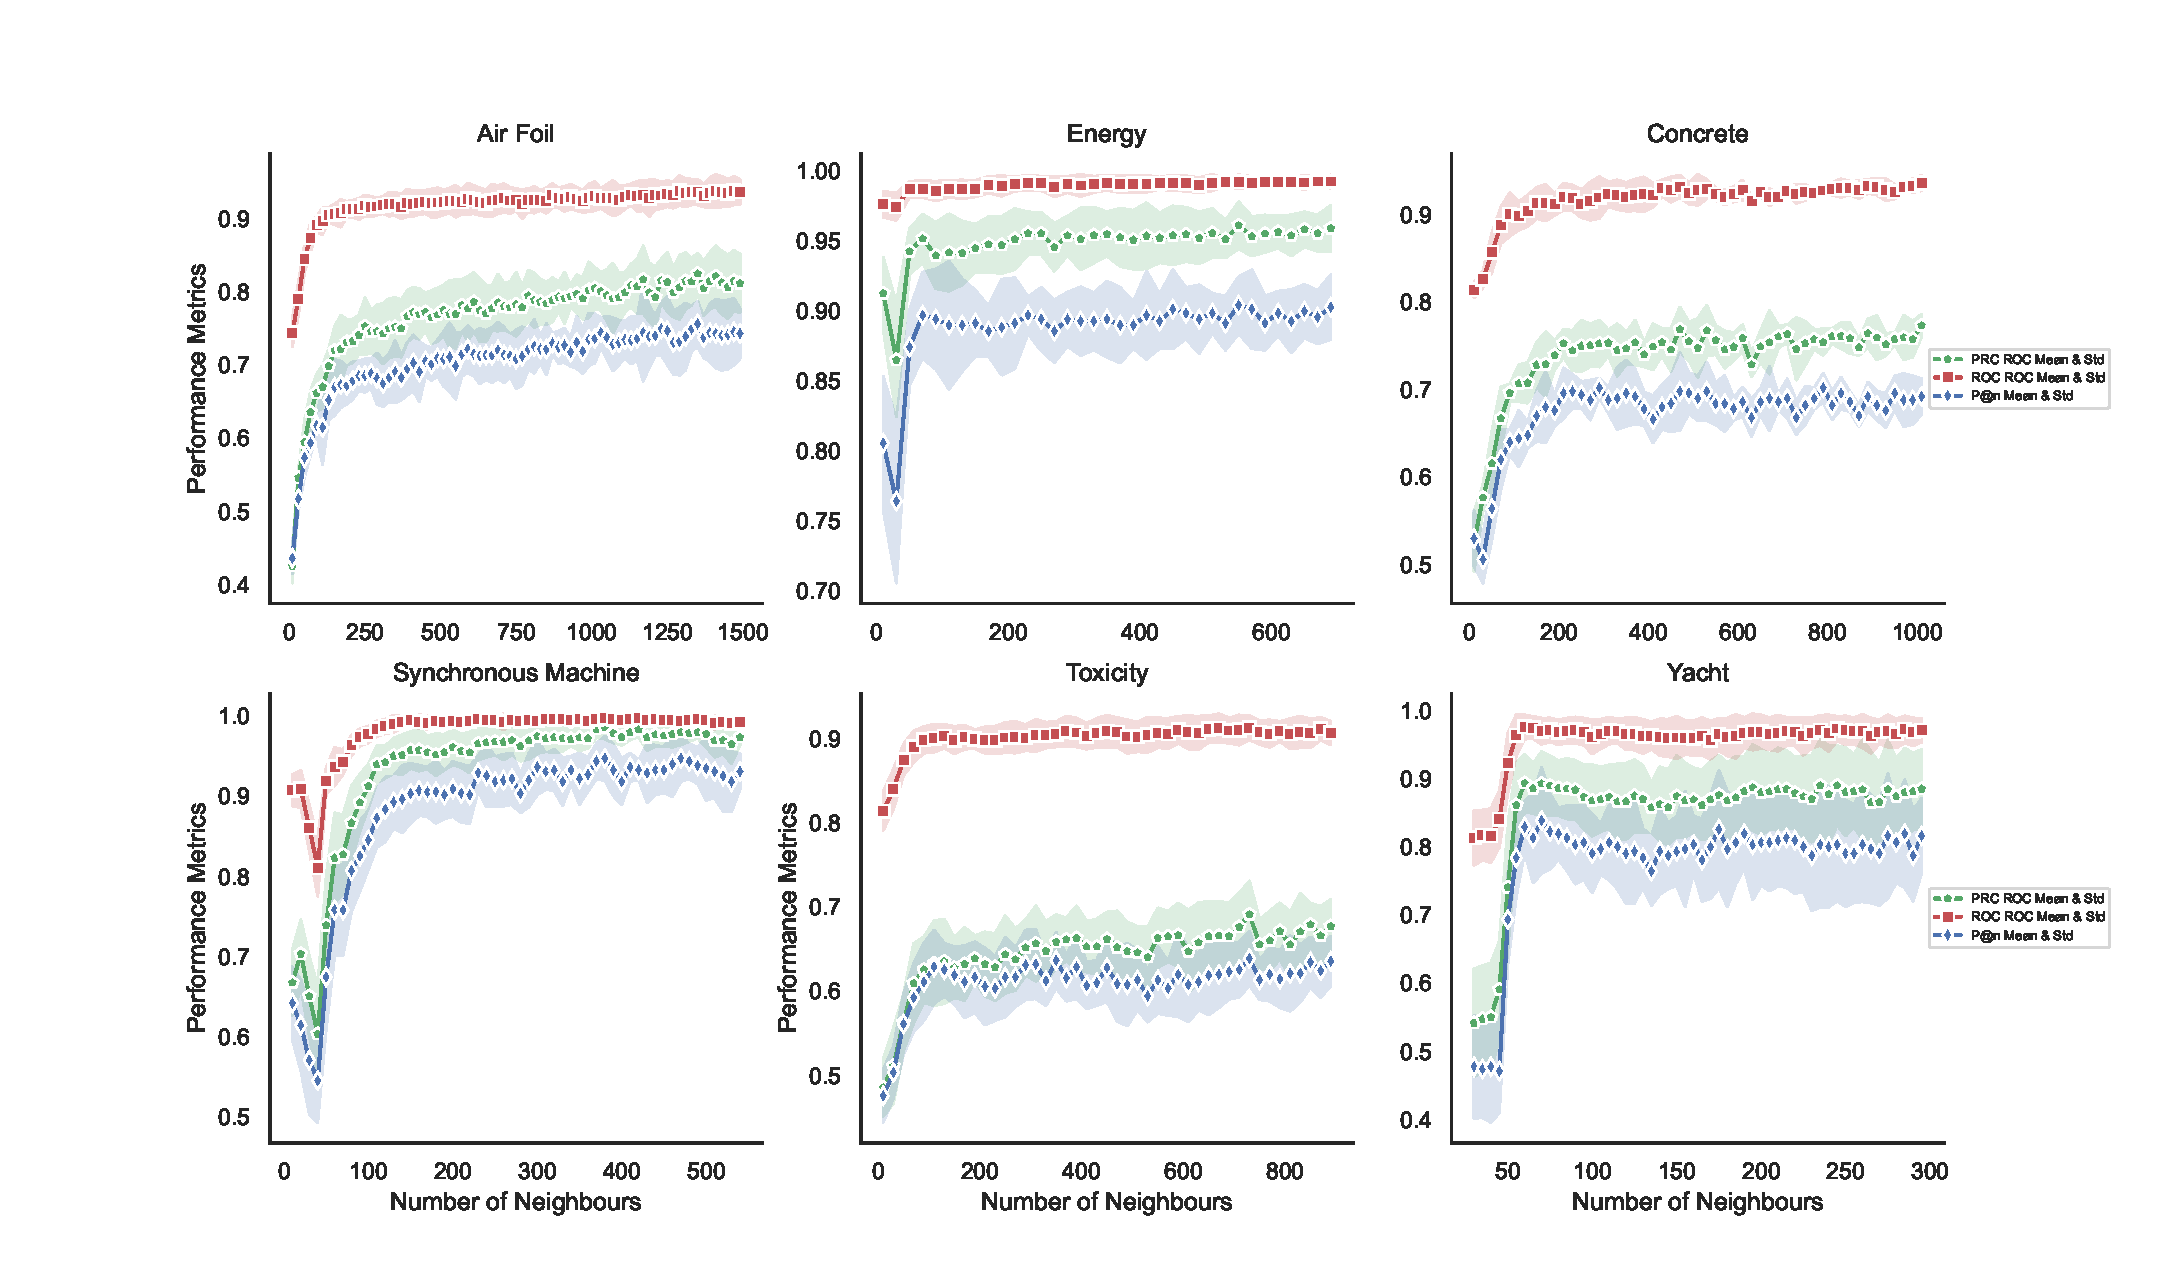
\includegraphics[width=12cm]{images/Pic_sensitivity1.pdf}
\caption{Phân tích độ nhạy trên tham số $k$, trong đó các đường biểu thị giá trị trung bình và các vùng được tô bóng biểu thị độ lệch chuẩn tương ứng của từng số liệu trong các thử nghiệm độc lập 10. Việc tăng số lượng hàng xóm trước tiên sẽ cải thiện phần lớn hiệu suất về mặt PRC AUC (đường màu xanh lá cây có dấu hoa thị), ROC AUC (đường màu đỏ có hình vuông) và Precision@n (đường màu xanh có hình kim cương), sau đó mang lại mức tăng hiệu suất không đáng kể. }\label{fig:sensitivity1}
\end{figure}
\section{Nghiên cứu cắt bỏ}
\label{Appendix:Ablation}
\subsection{Tỷ lệ độ dài khoảng thời gian phân vị có điều kiện}

Trong phần phương pháp của chúng tôi, chúng tôi đã xác định độ dài khoảng phân vị có điều kiện phù hợp cho một quan sát $b^{q}$ khi $b^{q} > \tau_{100}^{q}$ hoặc $ b^{q} <\tau_{0}^{q}$ như trong Phương trình (4). Chúng tôi xác định độ dài khoảng phù hợp cho $b^{q}$ dựa trên $\mathrm{max}(w(\mathbf{x}\rvert\mathbf{b}^{q}))$ và mở rộng quy mô hơn nữa bằng cách xem xét khoảng cách của nó với $\tau_{100}^{q}$ hoặc $\tau_{0}^{q}$. Ngoài ra, chúng ta có thể chỉ cần xác định độ dài khoảng phù hợp là $\mathrm{max}(w(\mathbf{x}\rvert\mathbf{b}^{q}))$ mà không cần chia tỷ lệ. Nói cách khác, chúng ta có thể coi tất cả các quan sát nằm bên ngoài $[\tau_{0}^{q}, \tau_{100}^{q}]$ là như nhau. Tuy nhiên, như được hiển thị trong Hình \ref{fig:ablation1}, điều này sẽ dẫn đến sự suy giảm hiệu suất lớn về PRC AUC và Precision@n đối với hầu hết các tập dữ liệu.Cụ thể, Hình \ref{fig:ablation1} cho thấy sự khác biệt của các chỉ số hiệu suất, tức là PRC ROC, ROC AUC và Precision@n giữa việc chia tỷ lệ $\mathrm{max}(w(\mathbf{x}\rvert\mathbf{b}^{q}))$ có xem xét khoảng cách đến $\tau_{100}^{q}$ hoặc $\tau_{0}^{q}$ và không chia tỷ lệ $\mathrm{max}(w(\mathbf{x}\rvert\mathbf{b}^{q}))$. Đối với tất cả các tập dữ liệu, sự khác biệt là tích cực.
Đặc biệt, những khác biệt này rất lớn về mặt PRC AUC và Precision@n đối với hầu hết các tập dữ liệu như Năng lượng, Viêm gan, Bệnh nhân Gan Ấn Độ, 5 tổng hợp và 10 tổng hợp. Do đó, điều quan trọng là xác định độ dài khoảng phù hợp bằng cách xem xét khoảng cách tương ứng từ $b^{q}$ đến $\tau_{100}^{q}$ hoặc $\tau_{0}^{q}$ khi $b^{q}> \tau_{100}^{q}$ hoặc $b^{q}<\tau_{0}^{q}$.

\begin{figure}[!htbp]
\centering
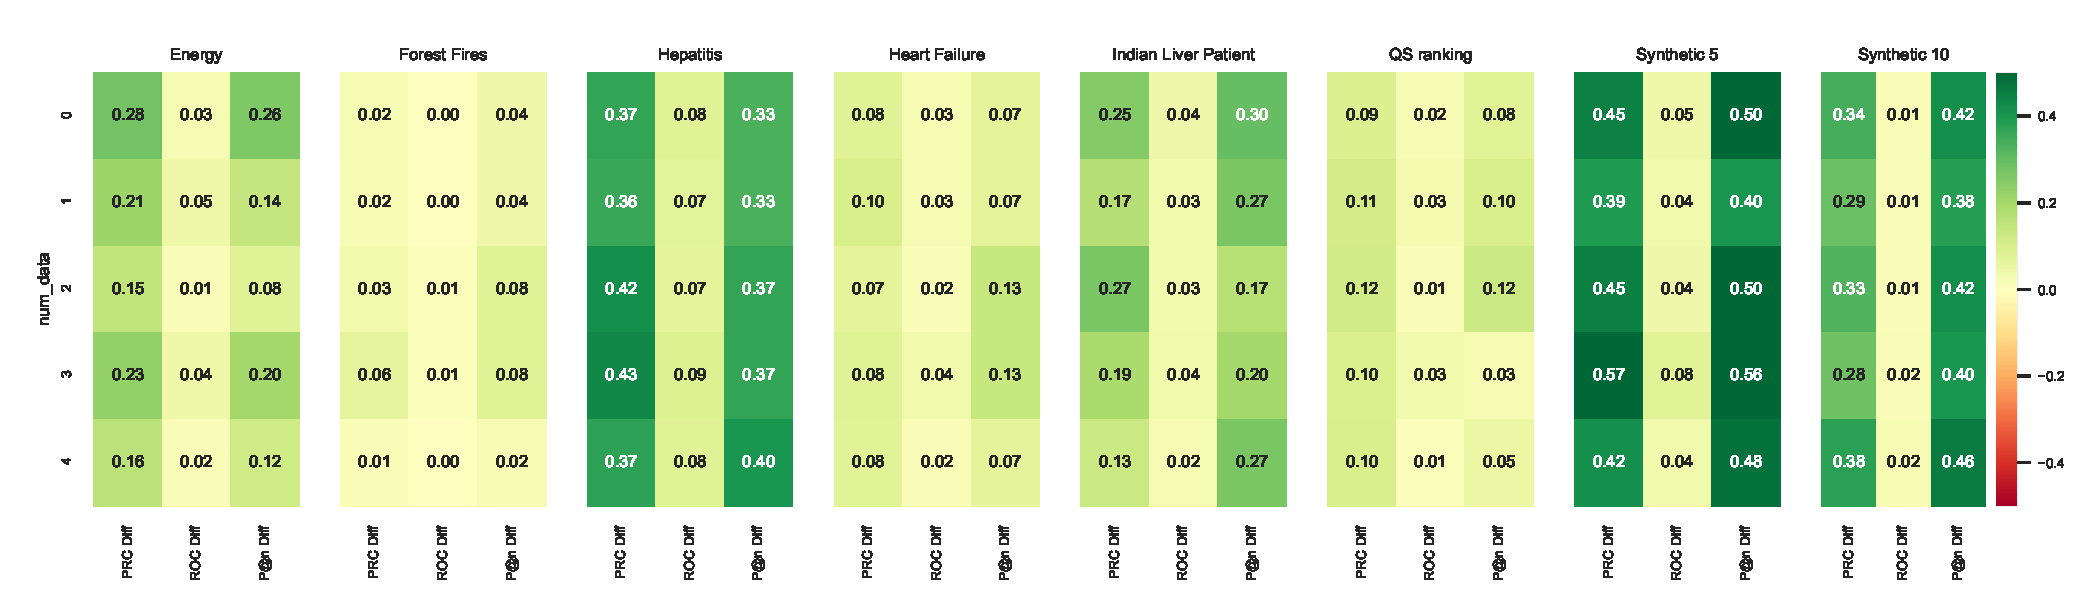
\includegraphics[width=12cm]{images/Pic_ablation1.pdf}
\caption{Hiệu ứng của việc chia tỷ lệ độ dài khoảng phân vị có điều kiện phù hợp. Đối với mỗi tập dữ liệu, kết quả thu được bằng cách thực hiện các thử nghiệm độc lập 5 về việc chèn các điểm bất thường theo ngữ cảnh. Đối với mỗi thử nghiệm, được biểu thị bằng trục y (cụ thể là $num\_data$), kết quả là sự khác biệt (theo PRC AUC, ROC AUC, Precision@n, tương ứng) của các phương pháp có hoặc không chia tỷ lệ độ dài khoảng phân vị có điều kiện phù hợp. Sự khác biệt lớn trên hầu hết các bộ dữ liệu cho thấy tầm quan trọng quan trọng của việc chia tỷ lệ độ dài khoảng cách phân vị có điều kiện phù hợp. }\label{fig:ablation1}
\end{figure}

\subsection{Cắt độ dài khoảng thời gian phân vị có điều kiện}
\begin{figure}[!htbp]
\centering
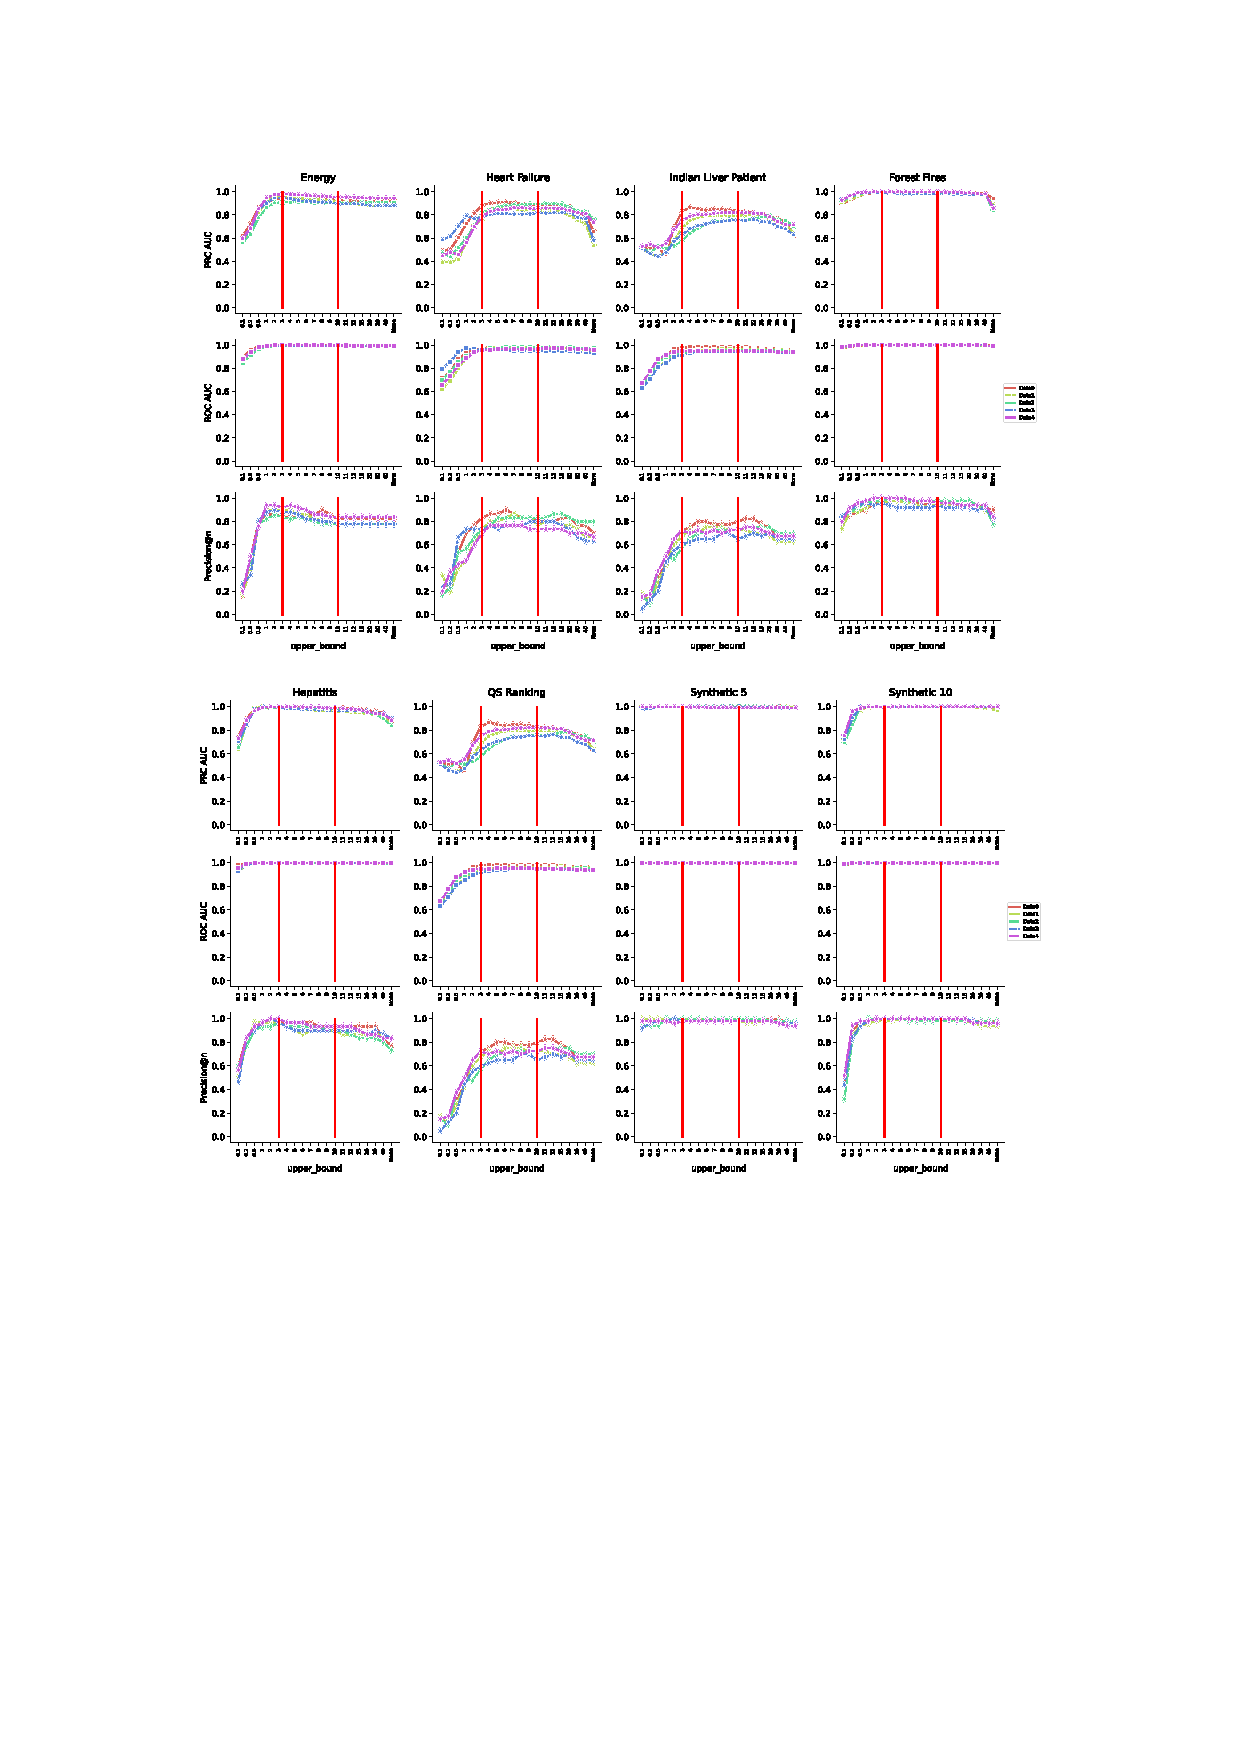
\includegraphics[width=12cm]{images/Pic_ablation2.pdf}
\caption{Hiệu ứng của việc cắt bớt độ dài khoảng phân vị có điều kiện phù hợp. Đối với mỗi tập dữ liệu, kết quả thu được bằng cách thực hiện các thử nghiệm độc lập 5 (được biểu thị bằng các đường cong khác nhau của 5) về việc chèn các bất thường theo ngữ cảnh. Sau đó, chúng tôi tính toán các số liệu hiệu suất (tức là PRC AUC, ROC AUC và Precision@n) của QCAD bằng cách thay đổi siêu tham số $\eta$ trong $\{0.1,0.2,0.5,1,2,3,...,11,12,15,20,30,40,None\}$, trong đó \textit{None} có nghĩa là không thực hiện cắt. Trên hầu hết các tập dữ liệu, hiệu suất tốt nhất đạt được khi sử dụng $3<\eta<10$, như được hiển thị bằng hai đường thẳng đứng màu đỏ.}\label{fig:ablation2}
\end{figure}

Để giảm thiểu \textit{hiệu ứng độc tài}, chúng tôi đã đề xuất cắt bớt độ dài khoảng phân vị có điều kiện phù hợp lớn với giới hạn trên, được đặt thành $\frac{\eta}{100}$. Cụ thể hơn, chúng tôi đặt $\eta=10$. Để chứng minh tính hiệu quả của chiến lược này trên các tập dữ liệu khác nhau, chúng tôi tính toán số liệu hiệu suất của QCAD bằng cách thay đổi siêu tham số $\eta \in \{0.1,0.2,0.5,1,2,3,...,11,12,15,20,30,40,None\}$, trong đó \textit{None} có nghĩa là không thực hiện cắt bớt.Như được hiển thị trong Hình \ref{fig:ablation2}, việc tăng $\eta$ sẽ dẫn đến các giá trị PRC AUC, ROC AUC và Precision@n cao hơn khi $\eta$ nhỏ (tức là nhỏ hơn $1$ đối với hầu hết các tập dữ liệu). Tiếp theo, một mặt, ROC AUC vẫn ổn định khi $\eta$ tăng, ngay cả khi không bị cắt (tức là $\eta=None$). Nói cách khác, chiến lược cắt bớt không ảnh hưởng đến số liệu ROC AUC. Mặt khác, PRC AUC và Precision@n dần dần đạt đến mức ổn định khi $\eta$ tăng lên. Sau một khoảng thời gian nhất định, PRC AUC và Precision@n bắt đầu giảm với mức tăng $\eta$. Nhìn chung, trên hầu hết các tập dữ liệu, PRC AUC và Precision@n thường đạt được giá trị cao hơn với $3\leq \eta \leq 10$ so với các tập dữ liệu không cắt bớt. Do đó, các hiệu ứng độc tài \textit{thực sự} tồn tại và chúng chủ yếu
giảm hiệu suất của QCAD về mặt PRC AUC và Precision@n. Hơn nữa, chiến lược cắt được đề xuất của chúng tôi có thể khắc phục vấn đề này một cách hiệu quả.
